   \documentclass{article}
\usepackage{pgfplots}
\begin{document}
\begin{figure}
\centering

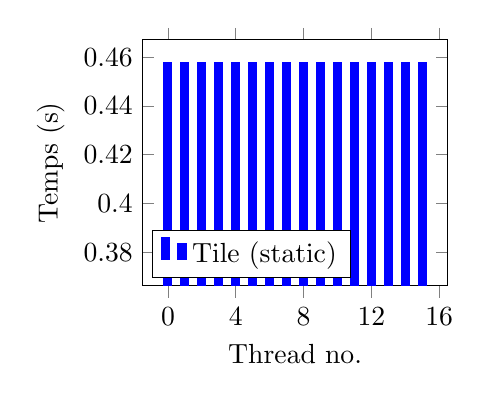
\begin{tikzpicture}
\begin{axis}[
  ybar,
  bar width=0.1cm,
  xlabel={Thread no.},
  ylabel={Temps (s)},
  ymin=.366210,
  legend pos=south west,
  width=0.45\textwidth,
  xtick distance=4
]

% Données pour le premier graphique (à gauche)
\addplot[color=blue, fill=blue] coordinates {
  (0,0.457785) (1,0.457803) (2,0.457787) (3,0.457788) (4,0.457781) (5,0.457778) (6,0.457769) (7,0.457786) (8,0.457781) (9,0.457763) (10,0.457933) (11,0.457949) (12,0.457815) (13,0.457795) (14,0.457795) (15,0.457815)
};
\addlegendentry{Tile (static)}

\end{axis}
\end{tikzpicture}
\hfill
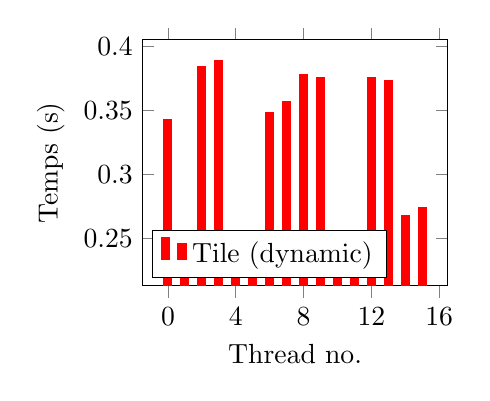
\begin{tikzpicture}
\begin{axis}[
  ybar,
  bar width=0.1cm,
  xlabel={Thread no.},
  ylabel={Temps (s)},
  ymin=,
  legend pos=south west,
  width=0.45\textwidth,
  xtick distance=4
]

% Données pour le deuxième graphique (au milieu)
\addplot[color=red, fill=red] coordinates {
  (0,0.343093) (1,0.246349) (2,0.384558) (3,0.389085) (4,0.229266) (5,0.230916) (6,0.348165) (7,0.356890) (8,0.377724) (9,0.375653) (10,0.235795) (11,0.238141) (12,0.375658) (13,0.373555) (14,0.268311) (15,0.274647)
};
\addlegendentry{Tile (dynamic)}

\end{axis}
\end{tikzpicture}
\hfill
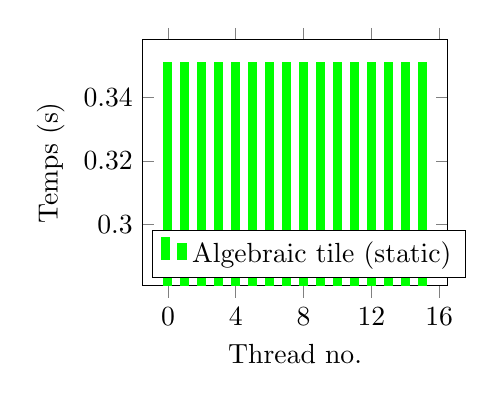
\begin{tikzpicture}
\begin{axis}[
  ybar,
  bar width=0.1cm,
  xlabel={Thread no.},
  ylabel={Temps (s)},
  ymin=.280751,
  legend pos=south west,
  width=0.45\textwidth,
  xtick distance=4
]

% Données pour le troisième graphique (à droite)
\addplot[color=green, fill=green] coordinates {
  (0,0.351055) (1,0.351070) (2,0.351065) (3,0.351083) (4,0.350939) (5,0.350977) (6,0.350944) (7,0.350982) (8,0.350974) (9,0.351011) (10,0.350994) (11,0.350990) (12,0.351127) (13,0.351130) (14,0.351052) (15,0.351094)
};
\addlegendentry{Algebraic tile (static)}

\end{axis}
\end{tikzpicture}

\caption{Temps d'exécution des threads pour le fichier 2mm.c}
\label{fig:graphes}
\end{figure}

\begin{table}[htbp]
  \centering
  \caption{Statistiques pour le fichier 2mm.c}
  \begin{tabular}{|c|c|c|c|}
    \hline
    Statistique & Algebraic Tile & Tile (static) & Tile (dynamic) \\ 
    \hline
    Skewness (g1) & 0.127666 & 1.98482 & -0.245877 \\ 
    Kurtosis (g2) & -1.21598 & 2.47571 & -1.73284 \\ 
    Écart type & 5.99103e-05 & 5.22754e-05 & 0.0631519\\ 
    Percent Imbalance metric en \% & 0.0284876 & 0.0307989 & 23.328\\ 
    Temps moyen (s) & 0.351130 & 0.457949 & 0.389085 \\ 
    \hline
  \end{tabular}
\end{table}
\newpage

\begin{figure}
\centering

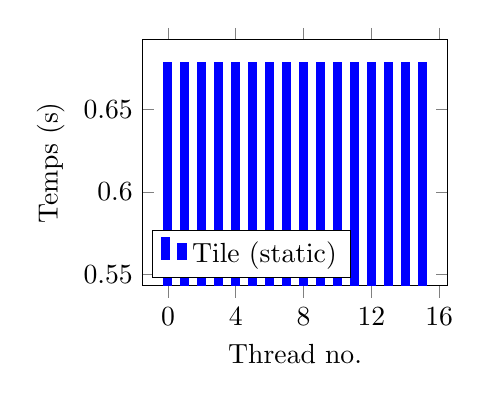
\begin{tikzpicture}
\begin{axis}[
  ybar,
  bar width=0.1cm,
  xlabel={Thread no.},
  ylabel={Temps (s)},
  ymin=.543001,
  legend pos=south west,
  width=0.45\textwidth,
  xtick distance=4
]

% Données pour le premier graphique (à gauche)
\addplot[color=blue, fill=blue] coordinates {
  (0,0.678806) (1,0.678845) (2,0.678805) (3,0.678844) (4,0.678764) (5,0.678764) (6,0.678756) (7,0.678791) (8,0.678776) (9,0.678773) (10,0.678752) (11,0.678791) (12,0.678800) (13,0.678760) (14,0.678780) (15,0.678779)
};
\addlegendentry{Tile (static)}

\end{axis}
\end{tikzpicture}
\hfill
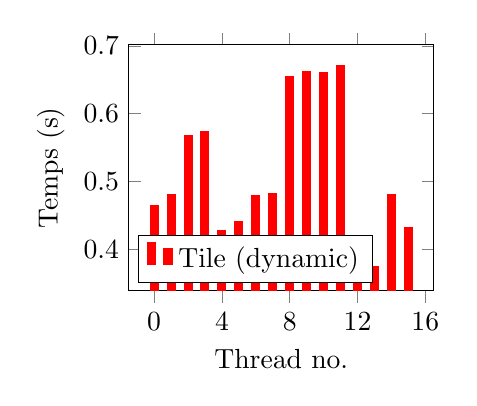
\begin{tikzpicture}
\begin{axis}[
  ybar,
  bar width=0.1cm,
  xlabel={Thread no.},
  ylabel={Temps (s)},
  ymin=,
  legend pos=south west,
  width=0.45\textwidth,
  xtick distance=4
]

% Données pour le deuxième graphique (au milieu)
\addplot[color=red, fill=red] coordinates {
  (0,0.465010) (1,0.480804) (2,0.567939) (3,0.573719) (4,0.427814) (5,0.441609) (6,0.479586) (7,0.482308) (8,0.654628) (9,0.661491) (10,0.661046) (11,0.671393) (12,0.369562) (13,0.374577) (14,0.480925) (15,0.432958)
};
\addlegendentry{Tile (dynamic)}

\end{axis}
\end{tikzpicture}
\hfill
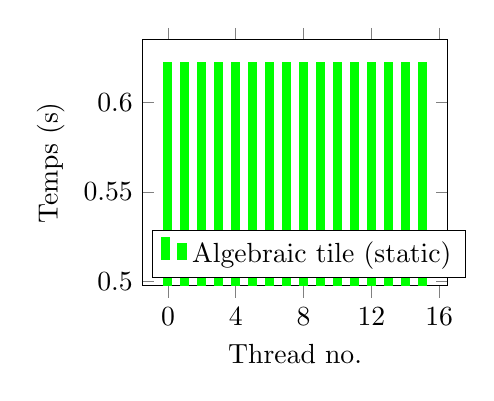
\begin{tikzpicture}
\begin{axis}[
  ybar,
  bar width=0.1cm,
  xlabel={Thread no.},
  ylabel={Temps (s)},
  ymin=.497644,
  legend pos=south west,
  width=0.45\textwidth,
  xtick distance=4
]

% Données pour le troisième graphique (à droite)
\addplot[color=green, fill=green] coordinates {
  (0,0.622055) (1,0.622085) (2,0.622062) (3,0.622089) (4,0.622162) (5,0.622119) (6,0.622171) (7,0.622218) (8,0.622333) (9,0.622315) (10,0.622275) (11,0.622334) (12,0.622265) (13,0.622227) (14,0.622209) (15,0.622267)
};
\addlegendentry{Algebraic tile (static)}

\end{axis}
\end{tikzpicture}

\caption{Temps d'exécution des threads pour le fichier 3mm.c}
\label{fig:graphes}
\end{figure}

\begin{table}[htbp]
  \centering
  \caption{Statistiques pour le fichier 3mm.c}
  \begin{tabular}{|c|c|c|c|}
    \hline
    Statistique & Algebraic Tile & Tile (static) & Tile (dynamic) \\ 
    \hline
    Skewness (g1) & -0.116693 & 0.884668 & 0.363687 \\ 
    Kurtosis (g2) & -1.29572 & -0.0472829 & -1.19499 \\ 
    Écart type & 9.31369e-05 & 2.72715e-05 & 0.100226\\ 
    Percent Imbalance metric en \% & 0.0216972 & 0.00854465 & 30.5994\\ 
    Temps moyen (s) & 0.622334 & 0.678845 & 0.671393 \\ 
    \hline
  \end{tabular}
\end{table}
\newpage

\begin{figure}
\centering

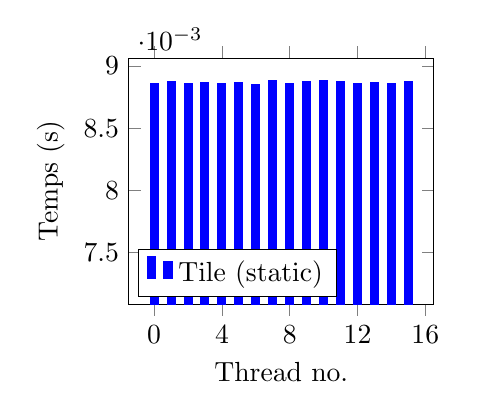
\begin{tikzpicture}
\begin{axis}[
  ybar,
  bar width=0.1cm,
  xlabel={Thread no.},
  ylabel={Temps (s)},
  ymin=.007083,
  legend pos=south west,
  width=0.45\textwidth,
  xtick distance=4
]

% Données pour le premier graphique (à gauche)
\addplot[color=blue, fill=blue] coordinates {
  (0,0.008860) (1,0.008872) (2,0.008857) (3,0.008869) (4,0.008857) (5,0.008869) (6,0.008854) (7,0.008879) (8,0.008858) (9,0.008871) (10,0.008883) (11,0.008871) (12,0.008858) (13,0.008870) (14,0.008859) (15,0.008871)
};
\addlegendentry{Tile (static)}

\end{axis}
\end{tikzpicture}
\hfill
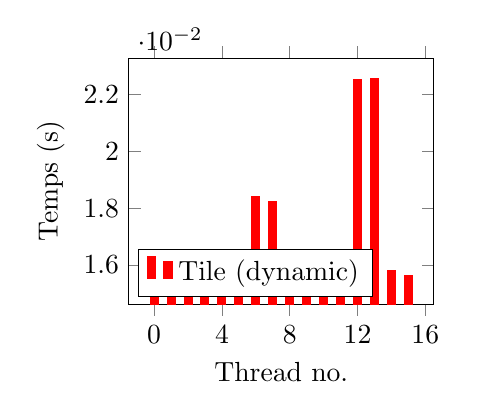
\begin{tikzpicture}
\begin{axis}[
  ybar,
  bar width=0.1cm,
  xlabel={Thread no.},
  ylabel={Temps (s)},
  ymin=,
  legend pos=south west,
  width=0.45\textwidth,
  xtick distance=4
]

% Données pour le deuxième graphique (au milieu)
\addplot[color=red, fill=red] coordinates {
  (0,0.015778) (1,0.015797) (2,0.015466) (3,0.015483) (4,0.015558) (5,0.015342) (6,0.018404) (7,0.018241) (8,0.015639) (9,0.015655) (10,0.015633) (11,0.015610) (12,0.022523) (13,0.022555) (14,0.015789) (15,0.015618)
};
\addlegendentry{Tile (dynamic)}

\end{axis}
\end{tikzpicture}
\hfill
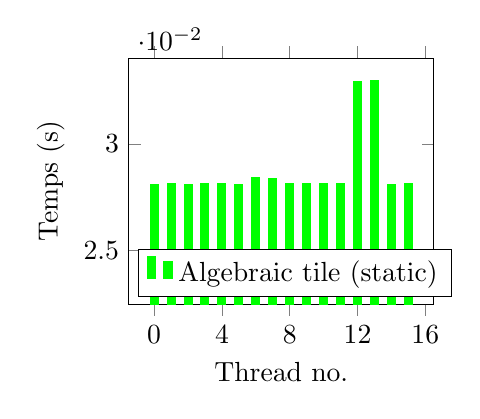
\begin{tikzpicture}
\begin{axis}[
  ybar,
  bar width=0.1cm,
  xlabel={Thread no.},
  ylabel={Temps (s)},
  ymin=.022470,
  legend pos=south west,
  width=0.45\textwidth,
  xtick distance=4
]

% Données pour le troisième graphique (à droite)
\addplot[color=green, fill=green] coordinates {
  (0,0.028108) (1,0.028134) (2,0.028115) (3,0.028138) (4,0.028135) (5,0.028106) (6,0.028401) (7,0.028379) (8,0.028129) (9,0.028159) (10,0.028142) (11,0.028147) (12,0.032939) (13,0.032982) (14,0.028088) (15,0.028121)
};
\addlegendentry{Algebraic tile (static)}

\end{axis}
\end{tikzpicture}

\caption{Temps d'exécution des threads pour le fichier mvt.c}
\label{fig:graphes}
\end{figure}

\begin{table}[htbp]
  \centering
  \caption{Statistiques pour le fichier mvt.c}
  \begin{tabular}{|c|c|c|c|}
    \hline
    Statistique & Algebraic Tile & Tile (static) & Tile (dynamic) \\ 
    \hline
    Skewness (g1) & 2.25439 & 0.279936 & 1.75427 \\ 
    Kurtosis (g2) & 3.10821 & -0.96557 & 1.54443 \\ 
    Écart type & 0.0015886 & 8.37313e-06 & 0.00233995\\ 
    Percent Imbalance metric en \% & 14.6646 & 0.190275 & 34.1107\\ 
    Temps moyen (s) & 0.032982 & 0.008883 & 0.022555 \\ 
    \hline
  \end{tabular}
\end{table}
\newpage

\begin{figure}
\centering

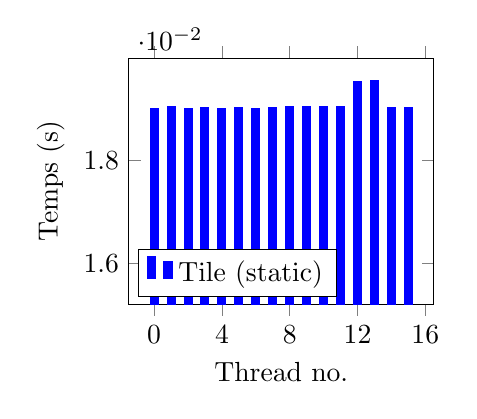
\begin{tikzpicture}
\begin{axis}[
  ybar,
  bar width=0.1cm,
  xlabel={Thread no.},
  ylabel={Temps (s)},
  ymin=.015210,
  legend pos=south west,
  width=0.45\textwidth,
  xtick distance=4
]

% Données pour le premier graphique (à gauche)
\addplot[color=blue, fill=blue] coordinates {
  (0,0.019013) (1,0.019055) (2,0.019021) (3,0.019033) (4,0.019014) (5,0.019027) (6,0.019014) (7,0.019027) (8,0.019060) (9,0.019047) (10,0.019047) (11,0.019060) (12,0.019548) (13,0.019559) (14,0.019037) (15,0.019025)
};
\addlegendentry{Tile (static)}

\end{axis}
\end{tikzpicture}
\hfill
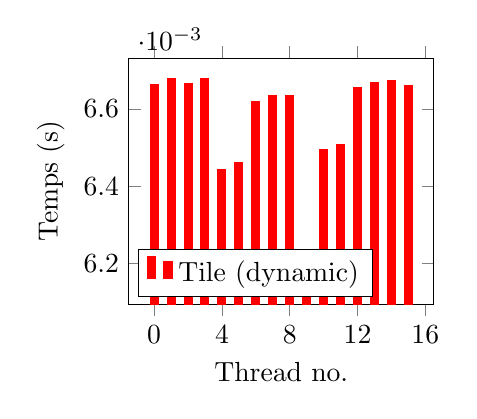
\begin{tikzpicture}
\begin{axis}[
  ybar,
  bar width=0.1cm,
  xlabel={Thread no.},
  ylabel={Temps (s)},
  ymin=,
  legend pos=south west,
  width=0.45\textwidth,
  xtick distance=4
]

% Données pour le deuxième graphique (au milieu)
\addplot[color=red, fill=red] coordinates {
  (0,0.006663) (1,0.006678) (2,0.006665) (3,0.006678) (4,0.006443) (5,0.006462) (6,0.006619) (7,0.006633) (8,0.006634) (9,0.006148) (10,0.006494) (11,0.006508) (12,0.006654) (13,0.006669) (14,0.006672) (15,0.006659)
};
\addlegendentry{Tile (dynamic)}

\end{axis}
\end{tikzpicture}
\hfill
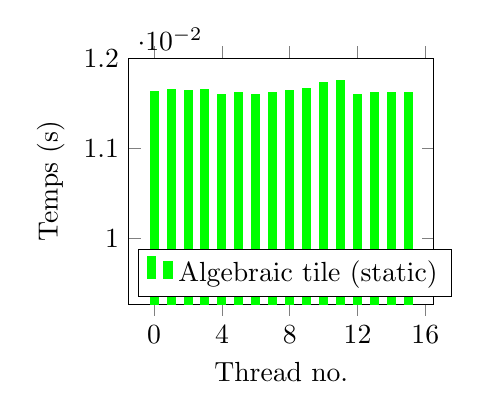
\begin{tikzpicture}
\begin{axis}[
  ybar,
  bar width=0.1cm,
  xlabel={Thread no.},
  ylabel={Temps (s)},
  ymin=.009274,
  legend pos=south west,
  width=0.45\textwidth,
  xtick distance=4
]

% Données pour le troisième graphique (à droite)
\addplot[color=green, fill=green] coordinates {
  (0,0.011632) (1,0.011654) (2,0.011638) (3,0.011658) (4,0.011599) (5,0.011622) (6,0.011596) (7,0.011617) (8,0.011644) (9,0.011666) (10,0.011732) (11,0.011753) (12,0.011593) (13,0.011620) (14,0.011624) (15,0.011618)
};
\addlegendentry{Algebraic tile (static)}

\end{axis}
\end{tikzpicture}

\caption{Temps d'exécution des threads pour le fichier mvt.c}
\label{fig:graphes}
\end{figure}

\begin{table}[htbp]
  \centering
  \caption{Statistiques pour le fichier mvt.c}
  \begin{tabular}{|c|c|c|c|}
    \hline
    Statistique & Algebraic Tile & Tile (static) & Tile (dynamic) \\ 
    \hline
    Skewness (g1) & 1.36647 & 2.23309 & -1.9413 \\ 
    Kurtosis (g2) & 1.10527 & 3.05713 & 3.36568 \\ 
    Écart type & 4.35099e-05 & 0.000172402 & 0.00013706\\ 
    Percent Imbalance metric en \% & 0.956913 & 2.40743 & 1.49029\\ 
    Temps moyen (s) & 0.011753 & 0.019559 & 0.006678 \\ 
    \hline
  \end{tabular}
\end{table}
\newpage

  \end{document}
